
\documentclass[11pt,a4paper]{article}
\usepackage[T1]{fontenc}
\usepackage{lmodern}
\usepackage{amsmath,amssymb,amsfonts,mathtools}
\usepackage{graphicx,booktabs,longtable,array,tabularx,adjustbox}
\usepackage{geometry,microtype,fancyhdr,lastpage,etoolbox,enumitem}
\usepackage{newunicodechar,textcomp}
\usepackage{hyperref}
\hypersetup{hidelinks,pdfcreator={XeLaTeX / QM1 academic edition}}
\geometry{left=20mm,right=20mm,top=22mm,bottom=23mm}
\setcounter{secnumdepth}{2}
\setlength{\parindent}{0pt}
\setlength{\parskip}{4pt plus 1pt}
\setlength{\emergencystretch}{2em}
\setlength{\tabcolsep}{3pt}
\renewcommand{\arraystretch}{1.16}
\setlist{nosep,topsep=3pt,itemsep=2pt,leftmargin=7mm}
\AtBeginEnvironment{longtable}{\footnotesize\setlength{\tabcolsep}{2.2pt}}
\newcommand{\tightlist}{\setlength{\itemsep}{0pt}\setlength{\parskip}{0pt}}
\providecommand{\Cov}{\operatorname{Cov}}
\providecommand{\Var}{\operatorname{Var}}
\providecommand{\Corr}{\operatorname{Corr}}
\providecommand{\MAD}{\operatorname{MAD}}
\providecommand{\E}{\mathbb{E}}
\providecommand{\R}{\mathbb{R}}
\newunicodechar{—}{\textemdash}
\newunicodechar{–}{\textendash}
\newunicodechar{€}{\texteuro}
\newunicodechar{≤}{\ensuremath{\leq}}
\newunicodechar{≥}{\ensuremath{\geq}}
\newunicodechar{×}{\ensuremath{\times}}
\newunicodechar{÷}{\ensuremath{\div}}
\newunicodechar{Σ}{\ensuremath{\Sigma}}
\newunicodechar{σ}{\ensuremath{\sigma}}
\newunicodechar{μ}{\ensuremath{\mu}}
\newunicodechar{Δ}{\ensuremath{\Delta}}
\newunicodechar{∑}{\ensuremath{\sum}}
\newunicodechar{≈}{\ensuremath{\approx}}
\newunicodechar{√}{\ensuremath{\surd}}
\newunicodechar{≠}{\ensuremath{\ne}}
\newunicodechar{→}{\ensuremath{\to}}
\newunicodechar{∞}{\ensuremath{\infty}}
\newunicodechar{∈}{\ensuremath{\in}}
\newunicodechar{−}{\ensuremath{-}}
\newunicodechar{²}{\ensuremath{^{2}}}
\newunicodechar{³}{\ensuremath{^{3}}}
\newunicodechar{₀}{\ensuremath{_{0}}}
\newunicodechar{₁}{\ensuremath{_{1}}}
\newunicodechar{₂}{\ensuremath{_{2}}}
\newunicodechar{₃}{\ensuremath{_{3}}}
\newunicodechar{₄}{\ensuremath{_{4}}}
\newunicodechar{ₜ}{\ensuremath{_{t}}}
\newunicodechar{ₚ}{\ensuremath{_{p}}}
\newunicodechar{ₙ}{\ensuremath{_{n}}}
\newunicodechar{ₓ}{\ensuremath{_{x}}}
\newunicodechar{ᵢ}{\ensuremath{_{i}}}
\newunicodechar{ŷ}{\ensuremath{\hat y}}
\newunicodechar{Ŷ}{\ensuremath{\widehat Y}}
\newunicodechar{ₘ}{\ensuremath{_{m}}}
\newunicodechar{ₑ}{\ensuremath{_{e}}}
\newunicodechar{ₐ}{\ensuremath{_{a}}}
\newunicodechar{ₖ}{\ensuremath{_{k}}}
\newunicodechar{ₛ}{\ensuremath{_{s}}}
\newunicodechar{ₗ}{\ensuremath{_{l}}}
\newunicodechar{ₕ}{\ensuremath{_{h}}}
\newunicodechar{ₒ}{\ensuremath{_{o}}}
\newunicodechar{₊}{\ensuremath{_{+}}}
\newunicodechar{₋}{\ensuremath{_{-}}}
\newunicodechar{₌}{\ensuremath{_{=}}}
\newunicodechar{₍}{\ensuremath{_{(}}}
\newunicodechar{₎}{\ensuremath{_{)}}}
\newunicodechar{⁻}{\ensuremath{^{-}}}
\newunicodechar{⁺}{\ensuremath{^{+}}}
\newunicodechar{⁰}{\ensuremath{^{0}}}
\newunicodechar{¹}{\ensuremath{^{1}}}
\newunicodechar{⁴}{\ensuremath{^{4}}}
\newunicodechar{⁵}{\ensuremath{^{5}}}
\newunicodechar{⁶}{\ensuremath{^{6}}}
\newunicodechar{⁷}{\ensuremath{^{7}}}
\newunicodechar{⁸}{\ensuremath{^{8}}}
\newunicodechar{⁹}{\ensuremath{^{9}}}
\makeatletter
\renewcommand{\section}{\@startsection{section}{1}{0pt}{2.0ex plus .7ex minus .3ex}{1.0ex}{\large\bfseries}}
\renewcommand{\subsection}{\@startsection{subsection}{2}{0pt}{1.8ex plus .5ex minus .2ex}{.7ex}{\normalsize\bfseries}}
\renewcommand{\subsubsection}{\@startsection{subsubsection}{3}{0pt}{1.3ex plus .4ex minus .2ex}{.5ex}{\normalsize\bfseries}}
\makeatother
\pagestyle{fancy}
\fancyhf{}
\renewcommand{\headrulewidth}{0.35pt}
\renewcommand{\footrulewidth}{0pt}
\fancyhead[L]{\small\textsc{KEDGE Business School --- QM1}}
\fancyhead[R]{\small\textsc{2026--2027}}
\fancyfoot[L]{\small Badr ABOUFARASSE, PhD}
\fancyfoot[R]{\small\thepage\ /\ \pageref{LastPage}}
\setlength{\headheight}{14pt}
\setkeys{Gin}{keepaspectratio}
\begin{document}

\begin{center}
{\small\textsc{KEDGE Business School \quad EBP1 \quad Quantitative Methods 1}}\\[6pt]
{\Large\bfseries Fiche 4 — Distributions bivariées et régression}\\[6pt]
{\normalsize\bfseries Corrigés intégralement détaillés}\\[6pt]
{\small Badr ABOUFARASSE, PhD \quad --- \quad 2026--2027}
\end{center}
\vspace{2mm}\hrule\vspace{6mm}

\hypertarget{applications-fondamentales}{%
\section{Applications fondamentales}\label{applications-fondamentales}}

Maîtriser les définitions et les calculs essentiels du cours.

\emph{Application du cours --- 15 min}

\hypertarget{exercice-3-droite-de-mayer}{%
\subsection{Exercice 3 -- Droite de Mayer}\label{exercice-3-droite-de-mayer}}

Pour les points {\((1,7),(2,10),(3,10),(4,14),(5,14)\)} : former deux sous-nuages, calculer leurs points moyens {\(A\)} et {\(B\)}, puis déterminer la droite de Mayer.

\hypertarget{corriguxe9-duxe9tailluxe9}{%
\subsubsection{Corrigé détaillé}\label{corriguxe9-duxe9tailluxe9}}

Premier sous-nuage : {\((1,7),(2,10),(3,10)\)} : {\[A=\left(\frac{1+2+3}{3},\frac{7+10+10}{3}\right)=(2,9).\]} Deuxième sous-nuage : {\((4,14),(5,14)\)} : {\[B=\left(\frac{4+5}{2},\frac{14+14}{2}\right)=(4.5,14).\]} {\[a=\frac{14-9}{4.5-2}=2,
\qquad
b=9-2(2)=5.\]} Donc : {\[\boxed{y=2x+5}.\]}

\hypertarget{construction-vuxe9rifiable-des-deux-points-moyens}{%
\subsubsection{Construction vérifiable des deux points moyens}\label{construction-vuxe9rifiable-des-deux-points-moyens}}

\begin{longtable}[]{@{}lllll@{}}
\toprule\noalign{}
Groupe & x & y & Moyenne x & Moyenne y \\
\midrule\noalign{}
\endhead
\bottomrule\noalign{}
\endlastfoot
A & 1, 2, 3 & 7, 10, 10 & 6/3=2 & 27/3=9 \\
B & 4, 5 & 14, 14 & 9/2=4.5 & 28/2=14 \\
\end{longtable}

\[a=(14-9)/(4.5-2)=2,\quad b=9-2\times2=5.\]

Contrôles : 2×2+5=9 et 2×4,5+5=14. La droite de Mayer n'est pas nécessairement la droite des moindres carrés.

\hypertarget{pruxe9paration-aux-uxe9valuations}{%
\section{Préparation aux évaluations}\label{pruxe9paration-aux-uxe9valuations}}

Résoudre des exercices de contrôle continu et de partiel en autonomie.

\emph{Préparation CC / partiel --- 35 min}

\hypertarget{exercice-1-ruxe9gression-linuxe9aire-compluxe8te}{%
\subsection{Exercice 1 -- Régression linéaire complète}\label{exercice-1-ruxe9gression-linuxe9aire-compluxe8te}}

On observe : {\[(1,3),\ (2,5),\ (3,5),\
(4,8),\ (5,9).\]}

\begin{enumerate}
\item
  Tracer le nuage de points et décrire direction, forme et intensité apparente.
\item
  Calculer {\(\bar x\)}, {\(\bar y\)}, {\(V(x)\)}, {\(V(y)\)}, {\(\Cov(x,y)\)} et le coefficient de corrélation {\(r\)}.
\item
  Estimer la droite des moindres carrés {\(\hat y=ax+b\)}.
\item
  Calculer les valeurs ajustées et les résidus {\(e_i=y_i-\hat y_i\)}.
\item
  Calculer {\(SSE\)}, {\(SST\)} et {\(R^2\)} ; interpréter {\(R^2\)}.
\end{enumerate}

\hypertarget{corriguxe9-duxe9tailluxe9-1}{%
\subsubsection{Corrigé détaillé}\label{corriguxe9-duxe9tailluxe9-1}}

{\[\bar x=3,
\qquad
\bar y=6.\]} {\[V(x)=\frac{(1-3)^2+(2-3)^2+(3-3)^2+(4-3)^2+(5-3)^2}{5}=2.\]} {\[V(y)=\frac{(3-6)^2+(5-6)^2+(5-6)^2+(8-6)^2+(9-6)^2}{5}=4.8.\]} {\[\Cov(x,y)=\frac{1}{5}\sum (x_i-\bar
x)(y_i-\bar y)=3.\]} {\[r=\frac{3}{\sqrt{2\times4.8}}\approx0.96825.\]} Pente et constante : {\[a=\frac{\Cov(x,y)}{V(x)}=\frac{3}{2}=1.5,\]} {\[b=\bar y-a\bar x=6-1.5(3)=1.5.\]} Donc : {\[\boxed{\hat
y=1.5x+1.5}.\]}

\begin{longtable}[]{@{}llllll@{}}
\toprule\noalign{}
{\(x_i\)} & 1 & 2 & 3 & 4 & 5 \\
\midrule\noalign{}
\endhead
\bottomrule\noalign{}
\endlastfoot
{\(y_i\)} & 3 & 5 & 5 & 8 & 9 \\
{\(\hat y_i\)} & 3 & 4.5 & 6 & 7.5 & 9 \\
{\(e_i\)} & 0 & 0.5 & -1 & 0.5 & 0 \\
\end{longtable}

{\[SSE=0^2+0.5^2+(-1)^2+0.5^2+0^2=1.5.\]} {\[SST=\sum(y_i-\bar y)^2=24.\]} {\[R^2=1-\frac{SSE}{SST}=1-\frac{1.5}{24}=0.9375.\]} Environ 93.75\% de la variation observée de {\(Y\)} autour de sa moyenne est associée à l'ajustement linéaire.

Tableau complet de calcul, avec résidus et carrés des résidus :

\begin{longtable}[]{@{}lllllllll@{}}
\toprule\noalign{}
xᵢ & yᵢ & xᵢ² & yᵢ² & xᵢyᵢ & ŷᵢ & eᵢ & eᵢ² & \\
\midrule\noalign{}
\endhead
\bottomrule\noalign{}
\endlastfoot
1 & 3 & 1 & 9 & 3 & 3 & 0 & 0 & \\
2 & 5 & 4 & 25 & 10 & 4.5 & 0.5 & 0.25 & \\
3 & 5 & 9 & 25 & 15 & 6 & -1 & 1 & \\
4 & 8 & 16 & 64 & 32 & 7.5 & 0.5 & 0.25 & \\
5 & 9 & 25 & 81 & 45 & 9 & 0 & 0 & \\
Σ & 15 & 30 & 55 & 204 & 105 & 30 & 0 & 1.5 \\
\end{longtable}

\[\bar x=15/5=3,\quad\bar y=30/5=6,\quad V(x)=55/5-3^2=2,\quad V(y)=204/5-6^2=4.8.\]

\[\operatorname{Cov}(x,y)=105/5-3(6)=3,\quad a=3/2=1.5,\quad b=6-1.5(3)=1.5.\]

\[SSE=0+.25+1+.25+0=1.5,\quad SST=24,\quad R^2=1-1.5/24=.9375.\]

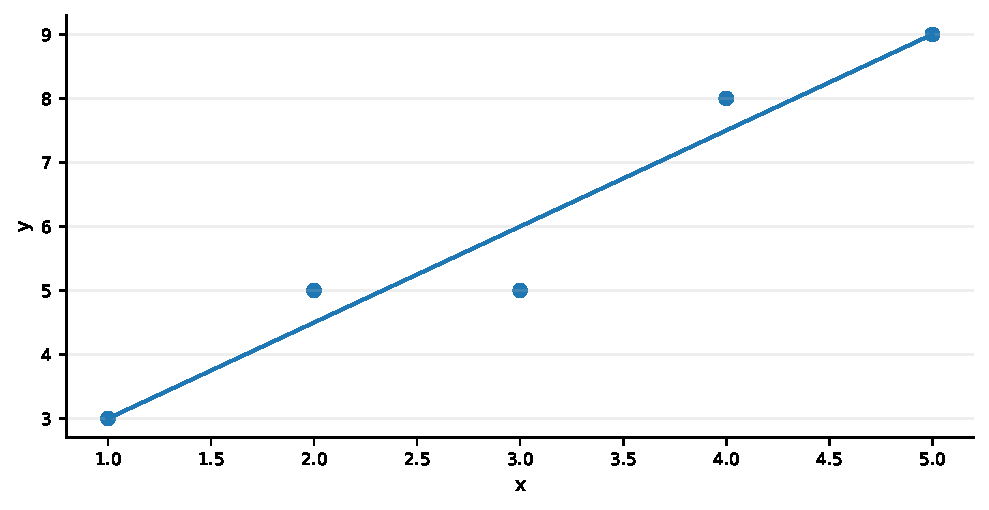
\includegraphics[width=0.82\textwidth,height=\textheight]{assets/chapter-4-solutions-fr-datachart-01.pdf}

\emph{Nuage de points / Scatter and OLS line}

\emph{Préparation CC / partiel --- 15 min}

\hypertarget{exercice-4-pruxe9vision-en-deux-uxe9tapes}{%
\subsection{Exercice 4 -- Prévision en deux étapes}\label{exercice-4-pruxe9vision-en-deux-uxe9tapes}}

\begin{longtable}[]{@{}lllllllll@{}}
\toprule\noalign{}
Mois & 1 & 2 & 3 & 4 & 5 & 6 & 7 & 8 \\
\midrule\noalign{}
\endhead
\bottomrule\noalign{}
\endlastfoot
Publicité {\(X\)} & 12 & 15 & 14 & 18 & 20 & 22 & 25 & 27 \\
Ventes {\(Y\)} & 48 & 52 & 50 & 59 & 63 & 68 & 73 & 78 \\
\end{longtable}

On donne les deux ajustements : {\[\widehat{Y}=2.064X+21.899,
\qquad
\widehat{X}_t=2.155t+9.429.\]} Prévoir la dépense publicitaire puis les ventes au mois 10. Identifier le caractère d'extrapolation de la première étape.

\hypertarget{corriguxe9-duxe9tailluxe9-2}{%
\subsubsection{Corrigé détaillé}\label{corriguxe9-duxe9tailluxe9-2}}

Au mois 10 : {\[\widehat
X_{10}=2.155(10)+9.429=30.979\approx30.98.\]} Cette valeur dépasse le maximum publicitaire observé, 27 : la première étape extrapole la tendance au-delà du mois 8.

La deuxième étape donne : {\[\widehat
Y_{10}=2.064(30.98)+21.899\approx85.84.\]} La prévision finale des ventes est donc d'environ 85.84 milliers d'euros.

\hypertarget{calcul-complet-des-deux-uxe9tapes}{%
\subsubsection{Calcul complet des deux étapes}\label{calcul-complet-des-deux-uxe9tapes}}

\begin{longtable}[]{@{}lllllllll@{}}
\toprule\noalign{}
t & 1 & 2 & 3 & 4 & 5 & 6 & 7 & 8 \\
\midrule\noalign{}
\endhead
\bottomrule\noalign{}
\endlastfoot
X & 12 & 15 & 14 & 18 & 20 & 22 & 25 & 27 \\
Y & 48 & 52 & 50 & 59 & 63 & 68 & 73 & 78 \\
\end{longtable}

\[\widehat X_{10}=2.155(10)+9.429=21.55+9.429=30.979.\]

\[\widehat Y_{10}=2.064(30.979)+21.899=63.940656+21.899=85.839656.\]

Le mois 10 est hors de l'intervalle observé 1--8 et la publicité prévue 30,979 est supérieure au maximum observé 27 : double extrapolation, à interpréter avec prudence.

\emph{Préparation CC / partiel --- 45 min}

\hypertarget{exercice-5-deux-ruxe9gressions-successives-type-partiel}{%
\subsection{Exercice 5 --- Deux régressions successives --- type partiel}\label{exercice-5-deux-ruxe9gressions-successives-type-partiel}}

Sur six périodes, on observe le rang t, la publicité x et les ventes y.

\begin{longtable}[]{@{}lllllll@{}}
\toprule\noalign{}
t & 1 & 2 & 3 & 4 & 5 & 6 \\
\midrule\noalign{}
\endhead
\bottomrule\noalign{}
\endlastfoot
x & 4 & 5 & 7 & 8 & 10 & 11 \\
y & 10 & 12 & 15 & 18 & 22 & 24 \\
\end{longtable}

\begin{enumerate}
\tightlist
\item
  Construire le tableau complet t, x, y, t², x², y², tx, xy et les sommes.
\item
  Calculer les moyennes, variances, covariance, r et la droite de x en fonction de t.
\item
  Faire de même pour y en fonction de x.
\item
  Prévoir x puis y pour t=8 ; qualifier les extrapolations.
\end{enumerate}

\hypertarget{corriguxe9-duxe9tailluxe9-3}{%
\subsubsection{Corrigé détaillé}\label{corriguxe9-duxe9tailluxe9-3}}

\begin{longtable}[]{@{}llllllll@{}}
\toprule\noalign{}
t & x & y & t² & x² & y² & t×x & x×y \\
\midrule\noalign{}
\endhead
\bottomrule\noalign{}
\endlastfoot
1 & 4 & 10 & 1 & 16 & 100 & 4 & 40 \\
2 & 5 & 12 & 4 & 25 & 144 & 10 & 60 \\
3 & 7 & 15 & 9 & 49 & 225 & 21 & 105 \\
4 & 8 & 18 & 16 & 64 & 324 & 32 & 144 \\
5 & 10 & 22 & 25 & 100 & 484 & 50 & 220 \\
6 & 11 & 24 & 36 & 121 & 576 & 66 & 264 \\
Σt=21 & 45 & 101 & 91 & 375 & 1853 & 183 & 833 \\
\end{longtable}

Régression de x sur t.

\[\bar t=21/6=3.5,\ \bar x=45/6=7.5,\ V(t)=91/6-3.5^2=2.916667,\ V(x)=375/6-7.5^2=6.25.\]

\[\begin{gathered}
\operatorname{Cov}(t,x)=183/6-3.5(7.5)=4.25,\\r_{tx}=\frac{4.25}{\sqrt{2.916667\times6.25}}=.995418.
\end{gathered}\]

\[a_1=4.25/2.916667=1.457143,\quad b_1=7.5-a_1(3.5)=2.4,\quad\widehat x_t=1.457143t+2.4.\]

Régression de y sur x.

\[\begin{gathered}
\bar y=101/6=16.833333,\\V(y)=1853/6-(101/6)^2=25.472222,\\\operatorname{Cov}(x,y)=833/6-(45/6)(101/6)=12.583333.
\end{gathered}\]

\[\begin{gathered}
r_{xy}=\frac{12.583333}{\sqrt{6.25\times25.472222}}=.997292,\\a_2=12.583333/6.25=2.013333,\\b_2=16.833333-a_2(7.5)=1.733333.
\end{gathered}\]

\[\begin{gathered}
\widehat y=2.013333x+1.733333,\\\widehat x_8=14.057143,\\\widehat y_8=2.013333(14.057143)+1.733333=30.035048.
\end{gathered}\]

t=8 dépasse la plage observée 1--6. Les deux étapes extrapolent ; aucune causalité n\textquotesingle est établie.

\hypertarget{approfondissement-facultatif}{%
\section{Approfondissement facultatif}\label{approfondissement-facultatif}}

Aller plus loin dans l'interprétation et les applications professionnelles.

\emph{Approfondissement --- 20 min}

\hypertarget{exercice-2-interpolation-extrapolation-causalituxe9-et-influence}{%
\subsection{Exercice 2 -- Interpolation, extrapolation, causalité et influence}\label{exercice-2-interpolation-extrapolation-causalituxe9-et-influence}}

À partir du modèle de l'exercice 1 :

\begin{enumerate}
\item
  prévoir {\(Y\)} pour {\(X=3.5\)} et qualifier la prévision ;
\item
  prévoir {\(Y\)} pour {\(X=10\)} et expliquer pourquoi cette prévision est risquée ;
\item
  ajouter le point {\((10,30)\)} et recalculer la pente et l'ordonnée à l'origine ; commenter l'influence de ce point ;
\item
  expliquer pourquoi une forte corrélation ne prouve pas une relation causale.
\end{enumerate}

\hypertarget{corriguxe9-duxe9tailluxe9-4}{%
\subsubsection{Corrigé détaillé}\label{corriguxe9-duxe9tailluxe9-4}}

Pour {\(X=3.5\)} : {\[\hat y=1.5(3.5)+1.5=6.75.\]} Comme {\(3.5\in[1,5]\)}, il s'agit d'une interpolation.

Pour {\(X=10\)} : {\[\hat y=1.5(10)+1.5=16.5.\]} Mais 10 est très au-delà du maximum observé 5 : c'est une extrapolation risquée.

Après ajout de {\((10,30)\)}, la nouvelle droite est approximativement : {\[\hat y=3.04918x-2.70492.\]} La pente passe de 1.5 à environ 3.05 : le point est très influent sur la droite ajustée. Une forte corrélation reste une mesure d'association ; elle ne suffit pas à établir une causalité, car des variables omises, une causalité inverse ou des mécanismes communs peuvent produire l'association.

Après ajout de (10,30), N=6, Σx=25, Σy=60, Σx²=155, Σy²=1104, Σxy=405.

\[V(x)=155/6-(25/6)^2=8.472222,\quad\operatorname{Cov}(x,y)=405/6-(25/6)(60/6)=25.833333.\]

\[a=25.833333/8.472222=3.049180,\quad b=10-3.049180(25/6)=-2.704918.\]

La pente passe de 1,50 à 3,05 : le point supplémentaire est influent.

\emph{Approfondissement --- 20 min}

\hypertarget{compluxe9ment-1-diagnostic-de-ruxe9gression-et-duxe9cision-responsable}{%
\subsection{Complément 1 --- Diagnostic de régression et décision responsable}\label{compluxe9ment-1-diagnostic-de-ruxe9gression-et-duxe9cision-responsable}}

Un modèle reliant fréquentation et température donne r = 0,78 et R² = 0,61. Le graphique des résidus est en U, un week-end d'été présente un résidu très élevé et le responsable veut prévoir une température supérieure de 12 °C au maximum observé.

\begin{enumerate}
\tightlist
\item
  Interprétez r et R².
\item
  Diagnostiquez les résidus.
\item
  Discutez le week-end atypique et la prévision.
\item
  Recommandez les étapes suivantes.
\end{enumerate}

\textbf{Indication méthodologique :}

Distinguez intensité, forme fonctionnelle, observation inhabituelle, extrapolation et causalité.

\hypertarget{corriguxe9-duxe9tailluxe9-5}{%
\subsubsection{Corrigé détaillé}\label{corriguxe9-duxe9tailluxe9-5}}

\textbf{Corrélation.} r = 0,78 décrit une association linéaire positive assez forte dans l'échantillon ; elle ne prouve pas la causalité.

\textbf{R².} Environ 61 \% de la variation observée de la fréquentation autour de sa moyenne est expliquée par la droite. Cela ne signifie pas que la température « cause 61 \% » de la fréquentation.

\textbf{Résidus.} Une forme en U révèle une courbure non prise en compte : la spécification linéaire est inadéquate.

\textbf{Week-end inhabituel.} Vérifier la donnée et rechercher festival, promotion ou fermeture. Comparer les estimations avec et sans ce point, sans le supprimer automatiquement.

\textbf{Extrapolation.} Prévoir 12 °C au-delà du maximum est très risqué, d'autant que la non-linéarité est visible.

\textbf{Suite.} Tester un terme quadratique ou une courbe flexible, valider hors échantillon, intégrer calendrier et promotions, mesurer l'influence et présenter l'incertitude.

\end{document}
